\section{Primary Cooling Loop (\emph{CoolSysPrimary}) - Chiller}\label{primary-cooling-loop-coolsysprimary---chiller}

The primary cooling system is constructed by using a \emph{PlantLoop} object. It uses an electric chiller that generates chilled water which is used to charge the TES tank at night. The chilled water stored in the TES tank is later used during the peak hours to satisfy the demand loads. Therefore, the supply side of the loop contains the electric chiller and the charge side of the TES tank. The demand side loop contains the cooling coil. The loop is operated by using plant equipment operation schemes, and schedules. Refer to Figure~\ref{fig:simple-line-diagram-for-the-primary-cooling} for a simple diagram of the Primary Cooling Loop.

\begin{figure}[hbtp] % fig 46
\centering
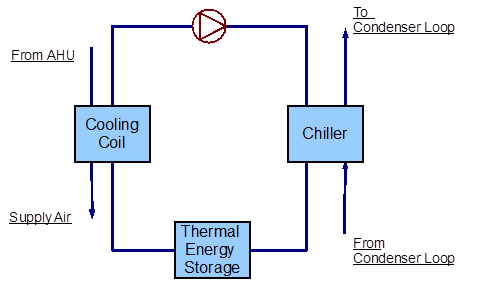
\includegraphics[width=0.9\textwidth, height=0.9\textheight, keepaspectratio=true]{media/image046.png}
\caption{Simple line diagram for the primary cooling system \protect \label{fig:simple-line-diagram-for-the-primary-cooling}}
\end{figure}

\subsection{Flowcharts for the Primary Cooling Loop Input Process}\label{flowcharts-for-the-primary-cooling-loop-input-process}

This series of flowcharts serve as a guide for identifying and inputting the CoolSysPrimary loop and its components into the input file. The working fluid in this loop is water. The important area for this loop is its controls. The EnergyPlus line diagram for this loop is provided in Figure~\ref{fig:energyplus-line-diagram-for-the-primary-001}. A simple flowchart for the separation of the half loops is provided in Figure~\ref{fig:simple-flowchart-for-the-separation-of-half-001}.

\begin{figure}[hbtp] % fig 47
\centering
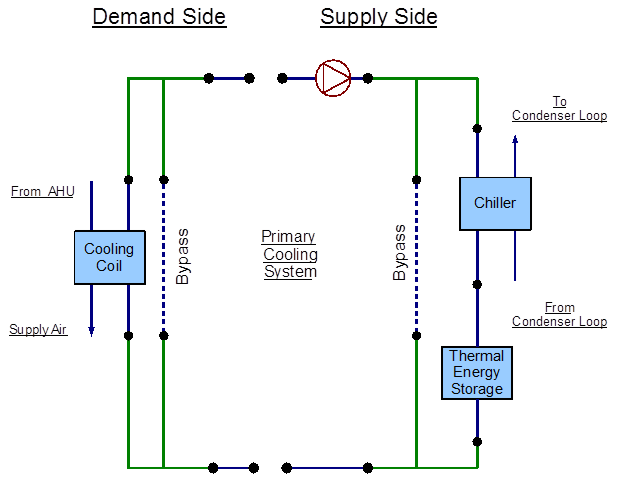
\includegraphics[width=0.9\textwidth, height=0.9\textheight, keepaspectratio=true]{media/image047.png}
\caption{EnergyPlus line diagram for the primary cooling system \protect \label{fig:energyplus-line-diagram-for-the-primary-001}}
\end{figure}

\begin{figure}[hbtp] % fig 48
\centering
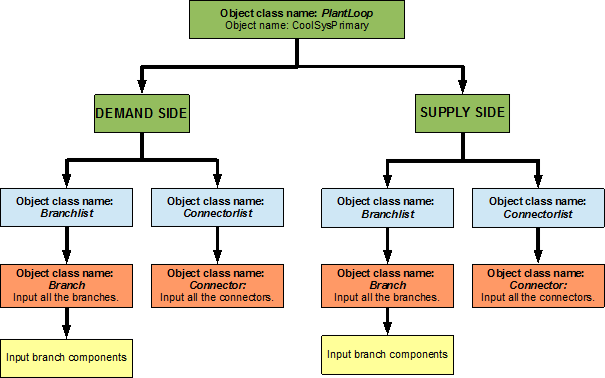
\includegraphics[width=0.9\textwidth, height=0.9\textheight, keepaspectratio=true]{media/image048.png}
\caption{Simple flowchart for the separation of half-loops in the primary cooling system \protect \label{fig:simple-flowchart-for-the-separation-of-half-001}}
\end{figure}

\subsubsection{CoolSysPrimary Supply Side Loop Construction}\label{coolsysprimary-supply-side-loop-construction}

The main components on the supply side half loop for the primary cooling system are the electric chiller that supplies the chilled water, the variable speed pump that circulates the chilled water through the loop, and the TES tank that stores the supplied chilled water. This half loop supplies chilled water to the cooling coil which is placed on the demand side half loop. The supply side half loop contains five components, four branches, nine nodes, and one splitter-mixer pair. The EnergyPlus line diagram for the primary cooling loop supply side is provided in Figure~\ref{fig:energyplus-line-diagram-for-the-supply-side-006}. The flowchart for supply side branches and components is provided in Figure~\ref{fig:flowchart-for-primary-cooling-loop-supply-side-branches}. The flowchart for supply side connectors is provided in Figure~\ref{fig:flowchart-for-primary-cooling-loop-supply-side-connectors}.

\begin{figure}[hbtp] % fig 49
\centering
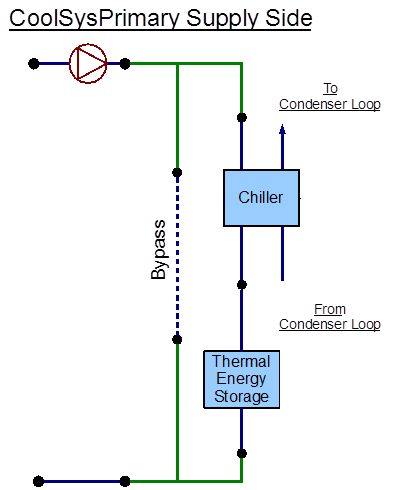
\includegraphics[width=0.9\textwidth, height=0.9\textheight, keepaspectratio=true]{media/image049.png}
\caption{EnergyPlus line diagram for the supply side of the primary cooling loop \protect \label{fig:energyplus-line-diagram-for-the-supply-side-006}}
\end{figure}

\begin{figure}[htbp] % fig 50
\centering
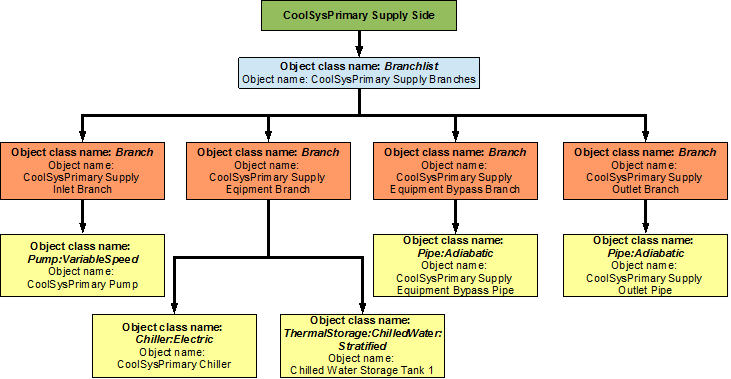
\includegraphics{media/image050.png}
\caption{Flowchart for primary cooling loop supply side branches and components \protect \label{fig:flowchart-for-primary-cooling-loop-supply-side-branches}}
\end{figure}

\begin{figure}[htbp] % fig 51
\centering
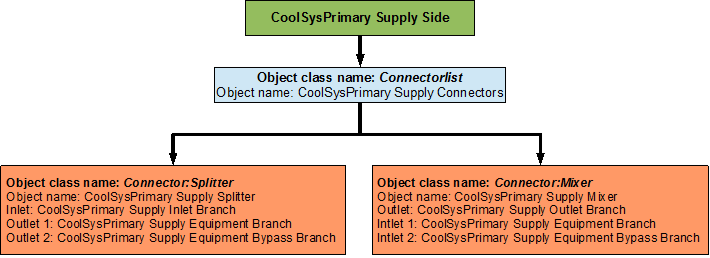
\includegraphics{media/image051.png}
\caption{Flowchart for primary cooling loop supply side connectors \protect \label{fig:flowchart-for-primary-cooling-loop-supply-side-connectors}}
\end{figure}

\subsubsection{CoolSysPrimary Demand Side Loop Construction}\label{coolsysprimary-demand-side-loop-construction}

The main component on the demand side half loop is the cooling coil which cools the air in the building by using the chilled water that is supplied by the supply side half loop. This side of the loop has eight nodes, four components, four branches, and one splitter mixer pair. An EnergyPlus line diagram for the demand side is provided in Figure~\ref{fig:energyplus-line-diagram-for-the-demand-side-006}. The flowchart for demand side branch definition is provided in Figure~\ref{fig:flowchart-for-primary-cooling-loop-demand-side-branches}. The flowchart for the demand side connectors is provided in Figure~\ref{fig:flowchart-for-primary-cooling-loop-demand-side-connectors}.

\begin{figure}[htbp] % fig 52
\centering
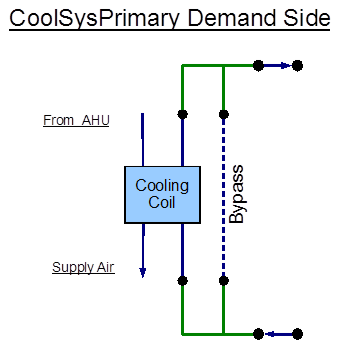
\includegraphics{media/image052.png}
\caption{EnergyPlus line diagram for the demand side of the primary cooling loop \protect \label{fig:energyplus-line-diagram-for-the-demand-side-006}}
\end{figure}

\begin{figure}[htbp] % fig 53
\centering
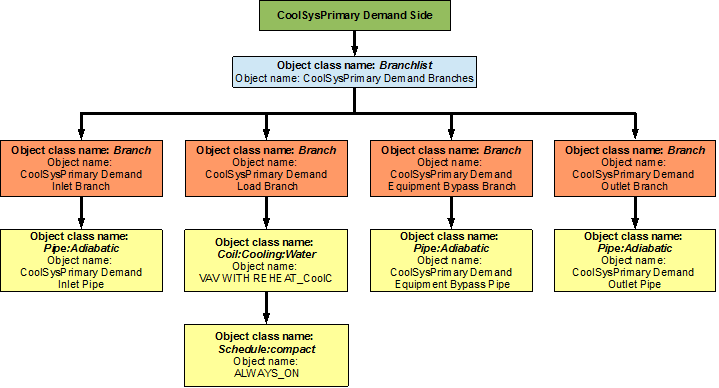
\includegraphics{media/image053.png}
\caption{Flowchart for primary cooling loop demand side branches and components \protect \label{fig:flowchart-for-primary-cooling-loop-demand-side-branches}}
\end{figure}

\begin{figure}[htbp] % fig 54
\centering
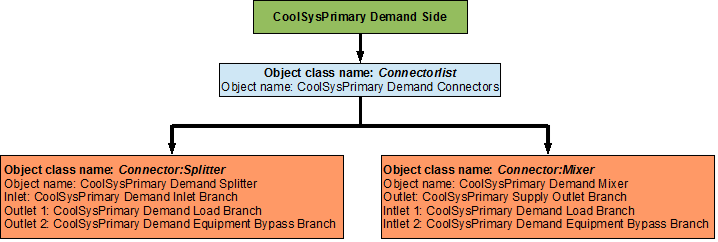
\includegraphics{media/image054.png}
\caption{Flowchart for primary cooling loop demand side connectors \protect \label{fig:flowchart-for-primary-cooling-loop-demand-side-connectors}}
\end{figure}

\subsection{Flowcharts for Primary Cooling Loop Controls}\label{flowcharts-for-primary-cooling-loop-controls}

The Primary Cooling loop is operated by using set-points, plant equipment operation schemes and schedules. The TES tank charging schedule is one of the most important schedules in this system.

\subsubsection{CoolSysPrimary Schedules}\label{coolsysprimary-schedules}

The flowchart for Primary Cooling loop schedule definition is provided in Figure 56. The Primary Cooling loop uses five different schedules to operate properly.~ The \emph{PlantOnSchedule} is a compact schedule that keeps the chiller and the TES tank ON at all times of the day, this compact schedule uses a discrete \emph{ScheduleTypeLimit} (\emph{On/Off)} which defines that the value of On is 1 and that of Off is 0. This plant loop also uses another compact schedule named \emph{CW Primary Loop Temp Schedule} declare that the temperature of the chilled water loop outlet flow is 6.7 degrees Celsius at all times. This schedule is used by the setpoint manager (\emph{CoolSysPrimary Loop Setpoint Manager)}. This schedule uses a schedule type limit named \emph{Temperature,} which defines the upper and lower loop temperature limits

The compact schedule \emph{ALWAYS\_ON} dictates that the use/discharge side of the TES tank is On at all times of the day. This schedule uses the \emph{ScheduleTypeLimit (Fraction)} to set the fractional flow rate of the use side. This schedule is used to define the use side availability of the TES tank. The compact schedule \emph{CW Tank Temp Schedule} is input in the TES tank object class to define the limits of the temperature for the chilled water storage tank outlet. This schedule uses the \emph{ScheduleTypeLimit (Temperature)} to define that the temperature at that outlet should be 7.5 degrees Celsius at all times of the day.

The \emph{TES Charge Schedule} is a very important schedule for the functioning of the CoolSysPrimary Loop the schedule from the input file is provided in Figure~\ref{fig:tes-charge-schedule}. The schedule shows that, the on/off \emph{ScheduleTypeLimit} is used to determine if the TES schedule is On or off for a certain period of time. A value of 1.0 means On and a value of 0 means Off. For example, it can be observed from the figure that, for the weekdays the TES tank is charged until 10:00AM, then it is operated during the day from 10:00 AM to 5:00 PM and then it is charged until midnight. The schedule for the other days is also shown in the figure.

\begin{figure}[hbtp] % fig 55
\centering
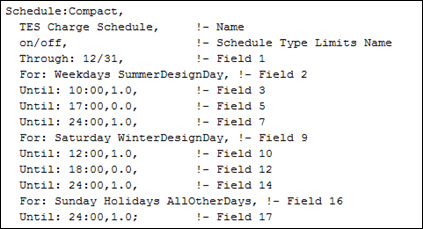
\includegraphics[width=0.9\textwidth, height=0.9\textheight, keepaspectratio=true]{media/image055.png}
\caption{TES Charge Schedule \protect \label{fig:tes-charge-schedule}}
\end{figure}

\begin{figure}[htbp] % fig 56
\centering
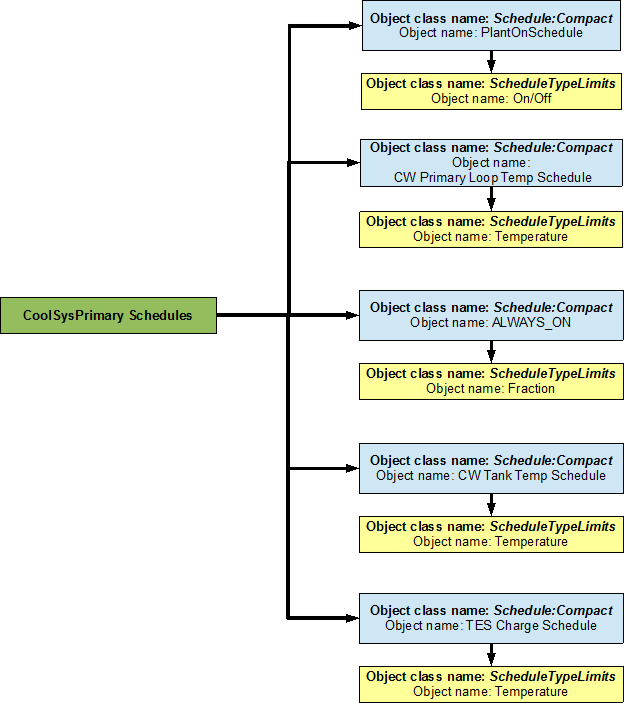
\includegraphics[width=0.9\textwidth, height=0.9\textheight, keepaspectratio=true]{media/image056.png}
\caption{Flowchart for primary cooling loop schedules \protect \label{fig:flowchart-for-primary-cooling-loop-schedules}}
\end{figure}

\subsubsection{CoolSysPrimary Plant Equipment Operation Schemes}\label{coolsysprimary-plant-equipment-operation-schemes}

This loop has two plant equipment operation schemes, one for the chiller and one for the TES tank. The \emph{PlantEquipmentOperationschemes} object uses the \emph{PlantOnSchedule} and the \emph{CoolSysPrimary Operation Scheme} objects to set the range of demand loads for which the chiller is operated during the simulation period. Operation schemes are especially useful and crucial when using multiple active components. For example, the performance of multiple chillers can be optimized by carefully managing the load ranges on each of the chillers. It should be noted that it is required to enter a plant equipment operation scheme for every plant loop in the system. A flowchart detailing the chilled water loop plant equipment operation schemes is provided in Figure~\ref{fig:flowchart-for-chiller-plant-equipment-operation}.

\begin{figure}[htbp] % fig 57
\centering
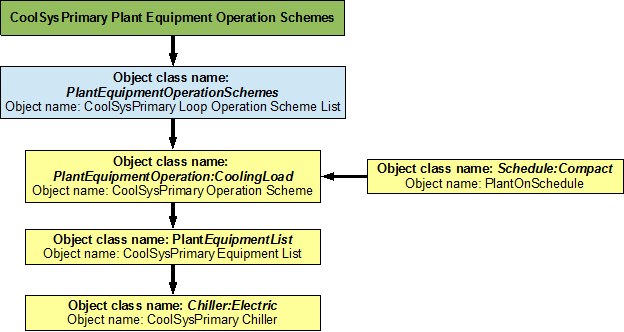
\includegraphics[width=0.9\textwidth, height=0.9\textheight, keepaspectratio=true]{media/image057.png}
\caption{Flowchart for Chiller plant equipment operation schemes \protect \label{fig:flowchart-for-chiller-plant-equipment-operation}}
\end{figure}

The TES tank operation is modeled here. The \emph{PlantEquipmentOperationschemes} object uses the \emph{PlantOnSchedule} and the \emph{TES Operation Scheme} objects to set the range of the demand loads for which the TES tank is operated during the simulation period. A flowchart detailing the Secondary Cooling Loop plant equipment operation schemes is provided in Figure~\ref{fig:flowchart-for-thermal-energy-storage-plant-equipment-operation}.

\begin{figure}[htbp] % fig 58
\centering
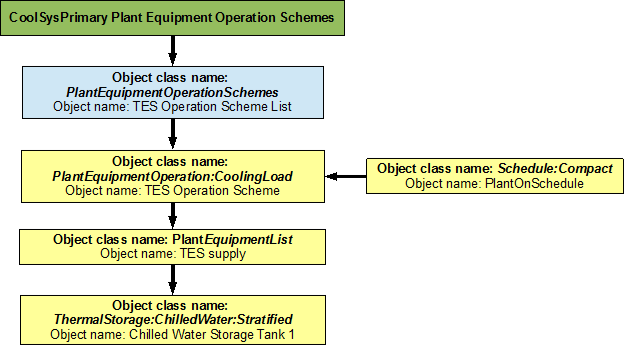
\includegraphics[width=0.9\textwidth, height=0.9\textheight, keepaspectratio=true]{media/image058.png}
\caption{Flowchart for Thermal Energy Storage plant equipment operation schemes \protect \label{fig:flowchart-for-thermal-energy-storage-plant-equipment-operation}}
\end{figure}

\subsubsection{CoolSysPrimary Setpoints}\label{coolsysprimary-setpoints}

The \emph{CoolSysPrimary Loop Setpoint Manager} uses the \emph{CoolSysPrimary Loop Temp Schedule} to set a temperature control point at the \emph{CoolSysPrimary Supply Outlet Node}. This setpoint allows the program to control the temperature at the node by operating the components in the Primary Cooling loop. ~A flowchart for Secondary Cooling loop setpoints is provided in Figure~\ref{fig:flowchart-for-primary-cooling-loop-setpoints-2016-06-17}.

\begin{figure}[htbp] % fig 59
\centering
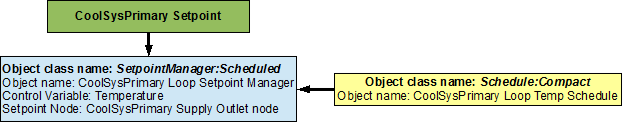
\includegraphics[width=0.9\textwidth, height=0.9\textheight, keepaspectratio=true]{media/image059.png}
\caption{Flowchart for primary cooling loop setpoints \protect \label{fig:flowchart-for-primary-cooling-loop-setpoints-2016-06-17}}
\end{figure}

\subsubsection{CoolSysPrimary Sizing}\label{coolsysprimary-sizing}

The chilled water loop is sized such a way that the design loop exit temperature is 6.7 degrees Celsius, and the loop design temperature difference is 5 degrees Celsius. A flowchart for the Secondary Cooling loop sizing is provided in Figure~\ref{fig:flowchart-for-primary-cooling-loop-sizing}.

\begin{figure}[htbp] % fig 60
\centering
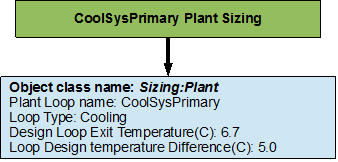
\includegraphics[width=0.9\textwidth, height=0.9\textheight, keepaspectratio=true]{media/image060.png}
\caption{Flowchart for primary cooling loop sizing \protect \label{fig:flowchart-for-primary-cooling-loop-sizing}}
\end{figure}
